\documentclass[titlepage]{article}

\usepackage[margin=1in]{geometry}
% some more shit for the title
\usepackage[T1]{fontenc}
\usepackage{babel}

% Tables and stopping them from displaying in a different section
\usepackage{booktabs}
\usepackage[section]{placeins}

% for inserting images into the document, setting file path, and allowing rotation of inserted images 
\usepackage{graphicx}
\graphicspath{ {./images/} }
\usepackage{rotating}
\usepackage[table]{xcolor}
% mostly just for putting text in math equations
\usepackage{amsmath}
% for aligning the text to the left
\usepackage[document]{ragged2e}

% for inserting hyperlinks in the document, use \url{url} or \href{url}{text}
\usepackage{hyperref}
\usepackage{calligra}
\usepackage[T1]{fontenc}
\usepackage{siunitx}
\usepackage{caption}
\usepackage{multirow}
\usepackage[export]{adjustbox}
\usepackage{tikz}
\usepackage{pgfplots}
\pgfplotsset{soldot/.style={color=black,only marks,mark=*},
	             holdot/.style={color=black,fill=white,only marks,mark=*},
		                  compat=1.12}
\usepackage{paracol}

\begin{document}
\title{\textbf{Lab 4: Resistivity of Nickel Chromium Wire and Use of the Wheatstone Bridge Circuit}}
\author{
    Zachary Pouska\\
    \texttt{001103193}\\
    \and
    Natalie Tran \\ 
    \texttt{000698629}\\ \\
    \and
    Joseph Pancho\\
    \texttt{002550975} \\ \\
} 

\date{PHYS 236 | Fall 2022\\
Date performed: 10/10/2022}


	\maketitle



	\section{Purpose}
	In this lab, we measured the resistance of a nickel chromium wire 
	and calculated the resistivity $\rho$. We then built a Wheatstone 
	bridge to find the resistances of individual capacitors.

	\section{Theory}
	Using nickel chromium wire $(80\%~Ni- 20\%~Cr)$, we will apply the 
	equations for calculating resistivity $\rho$. \\
	~\\
	For a given wire resistivity $\rho$, length $L$, and cross-sectional 
	area $A$, the resistance $R$, is given by: \\
	\[
		R=\frac{\rho L}{A}
	\]
	Solving for $\rho$, the above equation is re-written as:
	\[
		\rho = \frac{RA}{L}
	\]	 
	Verifying the untis for $\rho$: 
	\[
		\rho=\frac{\Omega m^2}{m}=\Omega m	
	\]
	\section{Experiment Analysis}
    



	\section{Procedure}
	For the first part of the lab, we first took six measurments of diameter 
	of the nichrome wire (mounted on a bridge-board) using calipers, two measurments per group member.
	Using the data, we then calculated cross-sectional area of the wire ($\pi r^2$) and resistivity 
	($\rho = \frac{RA}{L}$), where $R$ is the resistance ($\Omega$) of the wire measured with a 
	digital multimeter, $A$ is the cross-sectional area, and $l$ is the length of the wire.  
	The resistivity we found was compared to the given range of resistivity of a 
	nichrome wire: ($1.10*10^{-6}~\Omega m~to~1.50*10^{-6}~\Omega m$). \\
	~\\  
	For the second part of the lab, we put together a wheatstone bridge circuit using 
	the nichrome wire bridge-board, a power supply, a digital multimeter, a decade 
	resistance box, six unique resistors (tested one at a time), and alligator clips.
	A diagram of the circuit is shown below: 

	\begin{center}
		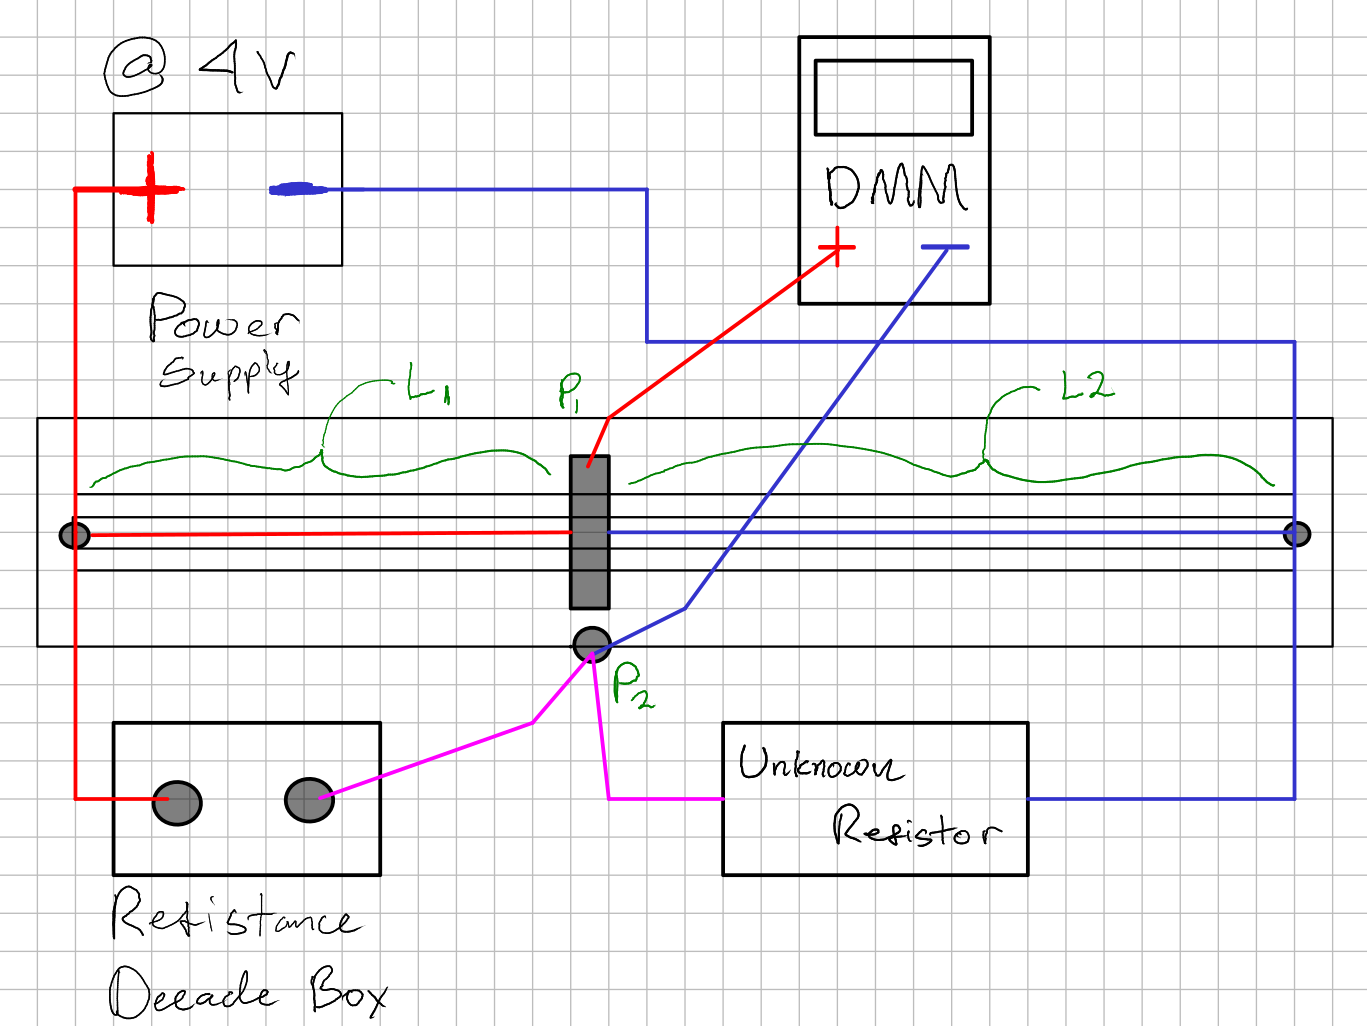
\includegraphics[scale=.2]{lab-circuit-diagram.png}
	\end{center}

	The digital multimeter's ground probe is afixed to a conductive screw on the edge of the 
	bridge-board $P_2$. The positive probe of the multimeter is free to move along the length 
	of the wire to find the where $V=0$, giving us lengths $L_1$ and $L_2$. Since the 
	resistances of the decade box and the unknown resistor are proportional to $L_1$ and $L_2$
	respectively, we can find the the value of the unknown resistance using:
	\[
		R_u=\frac{R_k L_2}{L_1}	
	\]
	Where $R_u$ is the unknown resistance and $R_k$ is the known resistance of the decade box. 
	

	\section{Data and Graphs}
	\subsection{Part 1}
	\subsection{Part 2} 
	\subsection{Part 3}
	\section{Results}
	\section{Questions}


	\subsection{Part 1}

	\subsection{Part 2}

    \subsection{Part 3}
	
    \subsection{Part 4}

	\section{Conclusion}

\end{document}
